\section{Energy-Dependent Model of the Probability for Electron Scattering within the \glsentryshort{wgts}}
\label{sec:appendixEDepScatCrossSecExtendedModel}
Section~\ref{sec:eDepScatCrossSecModel} introduces a model for the probability of electron scattering within the \gls{wgts} using the Poisson distribution. As explained, depending on the required accuracy, the conditions for using a Poisson distribution might be violated. Section~\ref{sec:appendixEDepScatCrossSecExtendedModelFormalism} introduces a model beyond the description via a Poisson distribution. Its evaluation was done numerically which demanded a trade-off between accuracy and run time. The latter is assessed in section~\ref{sec:appendixEDepScatCrossSecExtendedModelNumEval}.
\subsection{Modeling}
\label{sec:appendixEDepScatCrossSecExtendedModelFormalism}
In the following, a model for for the probability of electron scattering within the \gls{wgts} that depends on the electrons energy is derived. The difficulty lies in the fact, that an electron that scatters looses energy and hence its probability to scatter a second time is different from the first time. The presented model is inspired by a model given in~\cite{Groh2015}, that treats a similar effect for a change of an electron's pitch angles due to scattering. 

The aim is to derive an expression $\bar{P}^{\star}_l(\Esource)$ that denotes the probability of $l$-fold scattering for a $\upbeta$ electron with a starting energy $\Esource$ averaged over all starting positions and pitch angles assuming a fixed energy loss $\epsilon$ per scattering.

The expected amount of scatterings for a $\upbeta$ electron when traveling  through the whole \gls{wgts} volume of length $d$ filled with a gas of constant density $\rho$ is (see equation~\ref{eq:intSpecModelExpectedScatteringCount})
\begin{equation}
    \mu(E,\thetaSource) =
    \frac{\sigma(E)\rho d}{\cos\thetaSource},
\end{equation}
where $E$ denotes the electron's kinetic energy; $\thetaSource$ the starting pitch angle; and $\sigma(E)$ the energy dependent scattering cross section.

In the developed model, the volume of the \gls{wgts} is divided into $N$ slices of equal width $w=L/N$. $N$ is chosen sufficiently large that the probability for a $\upbeta$ electron to scatter twice within one slice is essentially zero. Then, for large $N$ the probability to scatter within one slice is $\mu(E,\thetaSource)/N$. The probability not to scatter within $n \leq N$ slices is
\begin{equation}
    p_0(E,\thetaSource,n) =
    \left(
        1-\frac{\mu(E,\thetaSource)}{N}
    \right)^n
    \fullstop
\end{equation}
Using the well known limit for the Euler constant, one obtains for $n=N$ and $N\rightarrow\infty$ that $p_0$ is a Poisson distribution with expectation $\mu$ evaluated at 0 
\begin{align}
    \lim_{N\rightarrow\infty} 
    p_0(E,\thetaSource,N) =
    \lim_{N\rightarrow\infty} 
    \left(
        1-\frac{\mu(E,\thetaSource)}{N}
    \right)^N =
    \mathrm{e}^{-\mu(E,\thetaSource)}
    \fullstop
\end{align}
In other words, for no scattering, the Poisson model for the scattering probabilities as described in section~\ref{sec:eDepScatCrossSecModel} is recovered.

Assuming a constant energy loss per scattering of $\epsilon$ the probability to scatter $l$ times within $n<N$ slices can be expressed recursively
\begin{equation}
	\label{eq:appendixEDepScatCrossSecExtendedModelFormalismCore}
    p_l(E,\thetaSource,n) =
    \underbrace{
        \sum_{k=l}^{n}
    }_{(4)}
    \underbrace{
        p_{l-1}(E,\thetaSource,k-1)
        \vphantom{\sum_{k=l}^{n}}
    }_{(1)}
    \underbrace{
    \left(
        1-p_0(E-(l-1)\epsilon,\thetaSource,1)
    \right)
    \vphantom{\sum_{k=l}^{n}}
    }_{(2)}
    \underbrace{
        p_0(E-l\epsilon,\thetaSource,n-k)
        \vphantom{\sum_{k=l}^{n}}
    }_{(3)}
    \fullstop
\end{equation}
The idea behind this expression is the following: One imagines an electron with an energy $E$ that travels through $n$ \gls{wgts} slices, scatters $l$ times in total and once in the $k$th slice. Hence, it must have scattered $l-1$ times in the $k-1$ slices and must not scatter in the $n-k$ slices to follow. In that regard, the above terms have the following meaning:
\begin{enumerate}[(1)]
    \item Probability to scatter $l-1$ times within $k-1$ slices with a kinetic energy of $E$.
    \item Probability to scatter once within the $k$th slice with a kinetic energy of $E-(l-1)\epsilon$.
    \item Probability not to scatter within the remaining $N-k$ slices.
    \item Sum over all slices $k$ where the electron could scatter the last time. The sum starts at $l$ because the probability to scatter $l-1$ times within less than $k=l-1$ slices (term (1)) is 0 because of the made assumption, that in the limit of large amount of slices $N$ an electron does not scatter twice within one very narrow slice.
\end{enumerate}
The probability to scatter $l$ times can be averaged over all starting positions
\begin{equation}
    \label{eq:appendixEDepScatCrossSecExtendedModelFormalismZAverage}
    \bar{p}_l(E,\thetaSource) = 
    \frac{1}{N}
    \sum_{\nSource=1}^{N} p_l(E,\thetaSource,\nSource) \approx
    \frac{1}{d}
    \int_{0}^{d}
        p_l(E,\thetaSource,
            \left\lceil N \frac{\zSource}{d}\right\rceil
        )
    \d \zSource
    \fullstop
\end{equation}
Here, the averaging sum is approximated by an integral as this helps cutting down on run time in a numerical evaluation. This is due to the fact, that in a numerical evaluation a large number $N$ ($\sim10^5$) of slices has to be chosen and the sum would have many terms. However, a numerical integration can achieve an accurate result with a smaller set of supporting points (see subsequent section~\ref{sec:appendixEDepScatCrossSecExtendedModelNumEval}). 

In the formal expression, the limit $N\rightarrow\infty$ can be applied
\begin{equation}
  P^{\star}_l(\Esource,\thetaSource) = 
    \lim_{N\rightarrow\infty} \bar{p}_l(\Esource,\thetaSource)
    \label{eq:appendixEDepScatCrossSecExtendedModelFormalismPitchAngleDepScatProbs}
\end{equation}
$P^{\star}_l(\Esource,\thetaSource)$ denotes the probability for a $\upbeta$ electron to scatter $l$ times when traveling through the whole \gls{wgts} with a starting energy $\Esource$ and pitch angle $\thetaSource$ averaged over all starting positions. Finally, this expression can be averaged over all starting pitch angles in order to obtain the energy dependent scattering probabilities
\begin{equation}
    \bar{P}^{\star}_l(\Esource) = 
    \frac{1}{1-\cos\thetaMax}
    \int_0^{\thetaMax}
    	\sin \thetaSource
        P^{\star}_l(\Esource,\thetaSource) 
        \d \thetaSource
    \fullstop
    \label{eq:appendixEDepScatCrossSecExtendedModelFormalismAveragedDepScatProbs}
\end{equation}
$\bar{P}^{\star}_l(\Esource)$ denotes the probability of $l$-fold scattering for a $\upbeta$ electron with a starting energy $\Esource$ averaged over all starting positions and pitch angles assuming a fixed energy loss $\epsilon$ per scattering. To derive such an expression was the aim of this section. 

\subsection{Numerical Evaluation and Cross-Check}
\label{sec:appendixEDepScatCrossSecExtendedModelNumEval}
\begin{figure}[t]
    \centering
    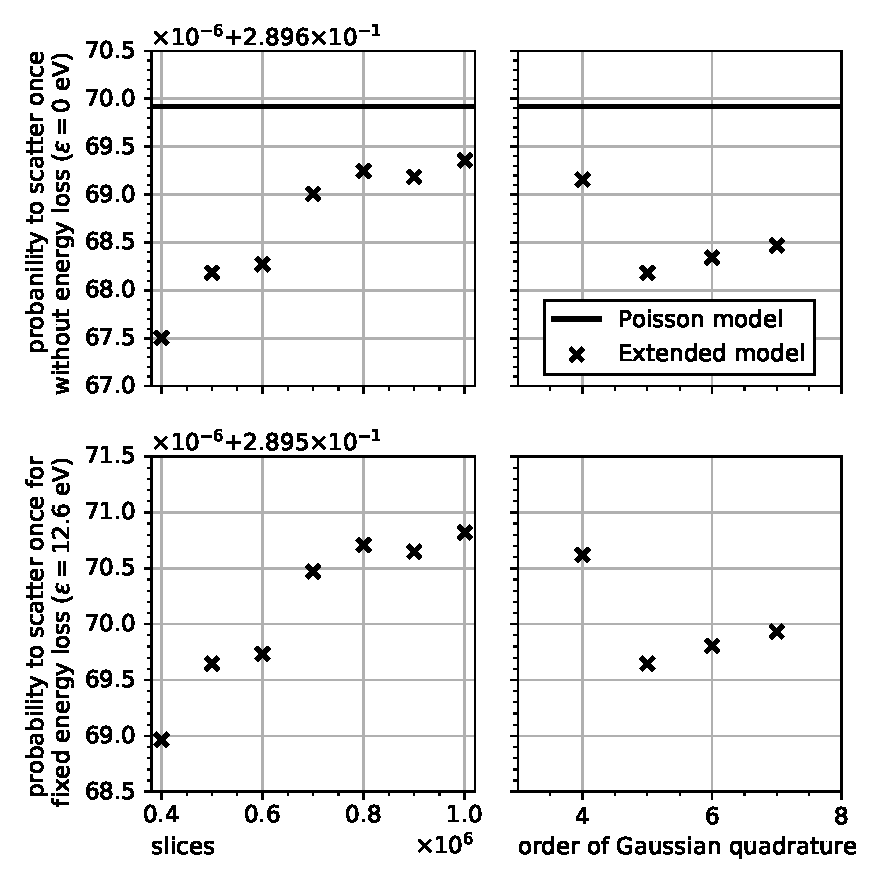
\includegraphics{chapter/energyDependentCrossSec/appendix/fig/scatProb1_numericalAccuracy.pdf}
    \xcaption{Numerical accuracy of the extended model for the probability for electron scattering within the \glsentryshort{wgts}}{Numerical accuracy of the extended model for the probability for electron scattering within the \glsentryshort{wgts}.}{The extended model is given by equation~\eqref{eq:appendixEDepScatCrossSecExtendedModelFormalismAveragedDepScatProbs} and the Poisson model is given by equation~\eqref{eq:eDepScatCrossSecModelPoisson}. For both models the energy of the incident electrons was taken as $\SI{18764.4}{eV}$ because for this energy, the Poisson model yields the values already given in table~\ref{tab:eDepScatCrossSecModelScatProbs}. The left column shows the dependence on the number $N$ of hypothetical slices of the \gls{wgts}. The right column shows the dependence on the order of Gaussian quadrature that was used to evaluate the two integrals in the extended model. The Poisson model is independent of these features and can be evaluated exactly (limited by machine number precision). In the left column the order of Gaussian quadrature was fixed to 5. In the right column the number of slices was fixed to $5\times10^{5}$. The upper row shows the numerical evaluation of the extended model for no energy loss per scattering (markers). Its exact solution is given by the Poisson model (line). The lower row shows the model for an energy loss of \SI{12.6}{eV} per scattering. The upper row shows that the numerical evaluation of the extended model is within a distance of $10^{-5}$ of its exact solution and the lower row shows conversion on the $10^{-5}$ level. These results make it plausible to assume a numerical inaccuracy on the $10^{-5}$ level for the shown configurations of the numerical evaluation.}
    \label{fig:appendixEDepScatCrossSecExtendedModelNumEval}
\end{figure}
The energy-dependent probability $\bar{P}^{\star}_l$ for electrons to scatter $l$-fold (extended model) in equation~\eqref{eq:appendixEDepScatCrossSecExtendedModelFormalismAveragedDepScatProbs} was evaluated numerically. Taking the limit~$N\rightarrow\infty$ in equation~\eqref{eq:appendixEDepScatCrossSecExtendedModelFormalismPitchAngleDepScatProbs} was replaced by choosing a large $N$. The averaging integral over the starting positions in equation~\eqref{eq:appendixEDepScatCrossSecExtendedModelFormalismZAverage} and starting pitch angles in equation~\eqref{eq:appendixEDepScatCrossSecExtendedModelFormalismAveragedDepScatProbs} was computed using Gaussian quadrature. The extended model was introduced because the preconditions to model the scattering probabilities via a Poisson distribution (Poisson model) do not hold. Hence, the numerical evaluation of the extended model must be sufficiently accurate to show the difference to the Poisson model. How accurate this is, can not be known beforehand and was found out by trial and error. Both, $N$ and the order of Gaussian quadrature, should be chosen as low as possible to cut down on run time, but sufficiently high for the required accuracy. 

Also, a benchmark had to be found, to determine the accuracy of the numerical evaluation. The following idea was used: For an energy loss of $\epsilon=\SI{0}{eV}$ per scattering, the extended model must recover the Poisson model exactly. This can be used to estimate the numerical accuracy in dependence of the number $N$ of slices and order of Gaussian quadrature. The estimated accuracy for $\epsilon=\SI{0}{eV}$ was then assumed for $\epsilon>\SI{0}{eV}$. A further cross-check is to look at the convergence of the numerical evaluation with increasing $N$ and an increasing order of the Gaussian quadrature.

The averaged probability for 1-fold scattering $\bar{P}^{\star}_1$ of the extended model, was evaluated for $\epsilon=\SI{0}{eV}$. The result in dependence of $N$ and the order of the Gaussian quadrature is shown in the top row of figure~\ref{fig:appendixEDepScatCrossSecExtendedModelNumEval}. It should recover th Poisson model. For $N=5\times10^5$ and using Gaussian quadrature of order 5, the Poisson model and the extended model differ less than $3\times10^{-6}$. Furthermore, the numerical calculation converges from below, which may be interpreted as a one-sided numerical inaccuracy. The calculations for $\epsilon=\SI{12.6}{eV}$ are shown in the lower row of figure~\ref{fig:appendixEDepScatCrossSecExtendedModelNumEval}. They also show convergence on the $10^{-5}$ level. Conclusively, the results make it plausible to assume a one-sided numerical inaccuracy on the $10^{-5}$ level for $N=10^5$ and using Gaussian quadrature of order 5 for the integrals.

The corresponding run time to compute $\bar{P}^{\star}_1$ is in $\mathcal{O}(N)$ as it requires a sum over all $N$ slices in equation~\ref{eq:appendixEDepScatCrossSecExtendedModelFormalismCore}. The extended model is defined recursively and therefore, the run time for $l$-fold scattering is in $\mathcal{O}(N^l)$. Hence, computing the probability for two-fold scattering would take $5\times10^5$ times as long as for one-fold scattering for the same $10^{-5}$ accuracy. This was not yet found to be feasible.
\FloatBarrier